
\vspace{-2pt}
\section{\benchname\xspace Benchmark}

\begin{table*}[t]
\centering
\small
\setlength{\tabcolsep}{3pt}
\renewcommand{\arraystretch}{1.15}

\resizebox{\textwidth}{!}{
\begin{tabular}{l p{1.0cm} c p{2.7cm} p{12cm}}
\toprule
\multirow{2}{*}{\makecell[l]{\textbf{Task}\\ \textbf{Name}}} &
\multirow{2}{*}{\makecell[c]{\hspace*{-10pt}\textbf{Memory}\\ \hspace*{-10pt}\textbf{Type}}} &
\multirow{2}{*}{\makecell[c]{\textbf{Avg.}\\ \textbf{\#Steps}}} &
\multirow{2}{*}{\makecell[l]{\textbf{Task}\\ \textbf{Challenge}}} &
\multirow{2}{*}{\makecell[l]{\textbf{Brief}\\ \textbf{Description}}} \\
& & & & \\
\midrule

% ================= Counting =================
\multicolumn{3}{l}{\texttt{Task Suite: \TSone}} &  \\

{PickXTimes} & T & 538 &  \text{count} &
Pick and place a cube of a given color for a specified number of repetitions. \\

\rowcolor{rowgray} BinFill & T & 604 & \text{count} &
Place a specified number of cubes of a given color into the bin as the cubes appear over time. \\


{SwingXTimes} & T & 435 & \text{count, swing-motion} &
Swing a cube back and forth between two targets for a specified number of cycles. \\

\rowcolor{rowgray}{StopCube} & T & 317 &\text{count, time-critical} &
Press a button \textit{exactly} when a moving cube reaches the target at a specified occurrence. \\

\midrule

% ================= Persistence =================
\multicolumn{3}{l}{\texttt{Task Suite: \TStwo}} &  \\
VideoUnmask & S & 217  & \text{occlusion} &
Given a video in which all cubes are masked, uncover the cube of a specified  color.\\
% with visually indistinguishable containers

\rowcolor{rowgray}ButtonUnmask & S & 267  & \text{occlusion} & 
Press the button, during which all cubes are masked, then uncover the cube of a specified  color.\\

VideoUnmaskSwap & S & 348  & \text{occlusion, tracking} &
Given a video in which all cubes are masked and containers dynamically swap positions, uncover the cube of a specified  color. \\

\rowcolor{rowgray}ButtonUnmaskSwap & S & 400 & \text{occlusion, tracking} &
Press the button, during which all cubes are masked and containers dynamically swap positions, then uncover the cube of a specified  color. \\

\midrule

% ================= Reference =================
\multicolumn{3}{l}{\texttt{Task Suite: \TSthree}} &  \\

PickHighlight & O & 346  & \text{visual-referential} &
Pick up all cubes that were visually highlighted in a short time during interaction. \\

\rowcolor{rowgray}
VideoRepick & O + T & 687  & \text{action-referential}, \text{tracking, count} &
Given a video showing a cube being manipulated and relocated, pick up the same cube for a specified number of repetitions.\\

VideoPlaceButton & O + T & 974  & \text{language-referential}, \text{long-video, tracking} &
Given a video with interleaved cube placement and button pressing, place the cube on the target specified by a language-described temporal reference (e.g., \textit{the target after pressing the button}). \\


\rowcolor{rowgray}
VideoPlaceOrder & O + T & 1134  & \text{language-referential}, \text{long-video, tracking} &
Given a video showing cube placement across multiple targets, place the cube on the target specified by a language-described ordinal reference (e.g., \textit{the second target}). \\


\midrule

% ================= Behavior =================
\multicolumn{3}{l}{\texttt{Task Suite: \TSfour}} &  \\
MoveCube & P & 394  & \text{contact-mode},\quad\quad \text{tool-use} &
Given a video showing cube transport, replicate the same demonstrated manipulation strategy (e.g., \textit{pick-and-place, pushing with the gripper, or hooking with a stick}).  \\

\rowcolor{rowgray} InsertPeg & P + O & 479  & \text{precise-motion} &
Given a video showing peg insertion, grasp the same peg at the same end and insert it into a box following the same demonstrated direction. \\


PatternLock & P & 208  & \text{linear-motion} &
Given a video showing a linear moving pattern, reproduce the same trajectory on the targets. \\

\rowcolor{rowgray} RouteStick & P & 370  &  \text{circular-motion} &
Given a video showing a circular routing pattern, reproduce the same trajectory around sticks. \\

\bottomrule
\end{tabular}}
% \vspace{0.05in}
\caption{\textbf{Task Summary}. Overview of all tasks, their corresponding memory types, average total timesteps, and key challenges. 
\label{tab:task_overview}
% The average number of steps includes the initial video frames for tasks conditioned on video inputs.
}
\end{table*}

% \vspace{0.2in}

\begin{table*}[t]
\centering
\small
\setlength{\tabcolsep}{3.5pt}
\resizebox{\textwidth}{!}{
\begin{tabular}{l|ccc|cc|cc|cccc}
\toprule
\multirow{2}{*}{\textbf{Dataset}} &
\multicolumn{3}{c|}{\textbf{Environment Complexity}} &
\multicolumn{2}{c|}{\textbf{Condition}} &
\multicolumn{2}{c|}{\textbf{Annotation}} &
\multirow{2}{*}[-0.5ex]{\makecell[c]{\textbf{Memory}\\ \textbf{Type}}} &
\multirow{2}{*}[-0.5ex]{\makecell[c]{\textbf{Total}\\ \textbf{\#Tasks}}} &
\multirow{2}{*}[-0.5ex]{\makecell[c]{\textbf{Total}\\ \textbf{\#Demos}}} &
\multirow{2}{*}[-0.5ex]{\makecell[c]{\textbf{Avg.}\\ \textbf{\#Steps}}} \\
\cmidrule(lr){2-4} \cmidrule(lr){5-6} \cmidrule(lr){7-8}
& \textbf{Non-Markov} & \textbf{Partial Obs.} & \textbf{Dynamic} 
 & \textbf{Vid.} & \textbf{Lang.} & \textbf{Subgoal} & \textbf{Keyframe}
& &  & \\
\midrule
RLBench18 \cite{james2020rlbench, shridhar2023perceiver}     & \xmark & \xmark & \xmark & \xmark & \cmark &  \xmark & \cmark &  T         & 18  & 1{,}800 & 137 \\
CALVIN \cite{mees2022calvin}        & \xmark & \xmark & \xmark  & \xmark & \cmark &   \cmark & \cmark & T         & 34  & 1{,}000 & 584 \\
LIBERO \cite{liu2023libero}        & \xmark & \xmark & \xmark  & \xmark & \cmark & \xmark & \xmark &  T         & 130 & 6{,}500 & 162 \\
VLABench \cite{zhang2025vlabench}      & \xmark & \xmark & \xmark & \xmark & \cmark & \xmark & \xmark &  T         & 100 & 1{,}600 & 115 \\
RoboCerebra \cite{han2025robocerebra}   & \xmark & \xmark & \cmark  & \xmark & \cmark & \cmark & \xmark &  T         & 100 & 1{,}000 & 2,972 \\

\midrule
% \textit{Memory-related benchmarks}  &  &  & & & & & &   &  & \\
MemoryBench \cite{fang2025sam2act}   & \cmark & \xmark & \xmark & \xmark & \cmark & \xmark & \cmark &  T+S       & 3   & 300 & 312\\
MIKASA-robo (VLA) \cite{cherepanov2025memory}   & \cmark & \cmark & \cmark  & \xmark & \xmark & \xmark & \xmark &  T+S+O     & 12  & 1,250 & 72 \\
\textbf{\benchname\xspace (Ours)} & \cmark & \cmark & \cmark & \cmark & \cmark & \cmark & \cmark &  \textbf{T+S+O+P} & \textbf{16} & \textbf{1{,}600} & \textbf{481} \\
\bottomrule
\end{tabular}}
% \vspace{0.05in}
\caption{
\textbf{Benchmark Comparison. }The upper section lists general-purpose benchmarks and the lower memory-based benchmarks. Memory types include temporal (T), spatial (S), object (O), and procedural (P). Environment complexity captures non-Markovian structure, partial observability, and dynamic scene change. 
Condition denotes initial inputs (Vid. for video observations; Lang. for language instructions). 
Annotations indicate the availability of language-based subgoals or keyframe timesteps for auxiliary supervision.
}
\label{tab:dataset_comparison}
\vspace{-8pt}
\end{table*}



% \begin{table*}[h]
% \centering


% \end{table*}

% In a standard Markov Decision Process, the optimal action at each step depends only on the current observation and action, as the state is assumed to fully summarize all relevant past information. Many existing robotic manipulation benchmarks are designed under this assumption, implicitly treating the environment as fully observable or Markovian.
% \benchname\xspace departs from this setting by focusing on non-Markovian manipulation scenarios. 


The aim of \benchname\xspace is to rigorously evaluate history-dependent behavior in robotic manipulation. 
All tasks are intentionally constructed to be non-Markovian, requiring models to reason over past observations that are no longer visible at the current step. 
Memory is essential for these tasks because identical observations can arise from different histories yet require different actions.



\subsection{Cognitively-Motivated Task Design}
% To evaluate history-dependent, long-horizon manipulation, we ground our task design in established cognitive models of human memory. Classical theories \cite{atkinson1968human} describe multiple forms of long-term memory, including procedural memory, which encodes motor skills acquired through practice \cite{squire2004memory}, and episodic memory, which supports recall of past events with their temporal order, spatial context, and object identity \cite{burgess2002human, hasselmo2017models, babb2011object}. We focus on these two forms because they align with the requirements of memory-augmented manipulation, motivating the four memory types defined below.
To systematically evaluate history-dependent, long-horizon manipulation, we ground our task design in established cognitive models of human memory. Classical theories \cite{atkinson1968human} divide long-term memory into \textit{procedural} and \textit{declarative} types, with declarative memory further divided into \textit{episodic} and \textit{semantic} forms. In particular, episodic memory supports recall of events and experiences, including temporal order, spatial context, and object identity \cite{burgess2002human, hasselmo2017models, babb2011object}, whereas procedural memory encodes motor skills acquired through practice \cite{squire2004memory}. Both are essential and relevant for memory-augmented manipulation, motivating the four memory types defined below.
% Drawing from these perspectives, we identify four core memory types most relevant to long-horizon robotic manipulation:

\begin{itemize}[itemsep=1pt, topsep=0pt, leftmargin=*]
\item \textbf{Temporal memory}: Tracks event counts, sequence ordering, and transition conditions across steps, e.g., determining when to proceed to the next subtask. 

\item \textbf{Spatial memory}: Maintains object locations and spatial relationships, especially when current visual information becomes unreliable due to occlusion or scene changes.

\item \textbf{Object memory}: Preserves referential consistency over time, enabling reliable object identification from visual, language, or action cues.

% \item \textbf{Procedural memory}: Enables replication of previously demonstrated behaviors, emphasizing action pattern replay rather than explicit factual recall\footnote{Procedural memory generally denotes skills and habits unconsciously acquired through extended practice (e.g., riding a bike). In this work, we focus on a narrower notion in manipulation: reproducing motion patterns from demonstrated videos.}.

\item \textbf{Procedural memory}: Reproduces previously demonstrated motion patterns or manipulation behaviors.

\end{itemize}

These four memory types correspond to the cognitive dimensions of when (temporal), where (spatial), what (object), and how (procedural).
\benchname\xspace is organized around these dimensions into four task suites, \TSone, \TStwo, \TSthree, \TSfour, each emphasizing a primary memory type for controlled evaluation.  Figure~\ref{fig:teaser} illustrates an overview of \benchname. Specifically, the \TSone\xspace suite targets \textit{temporal memory} by requiring agents to repeat actions a specified number of times, including pick-and-place, linear swinging, and time-critical  tasks. 
The \TStwo\xspace suite focuses on \textit{spatial memory}, evaluating object location tracking from pre-recorded videos or during concurrent manipulation.
The \TSthree\xspace suite evaluates \textit{object memory} through persistent identity resolution under visual, action-based, and language-based referential cues.
The \TSfour\xspace suite targets \textit{procedural memory} by requiring agents to reproduce demonstrated motion patterns, such as pushing, inserting, and sequential linear or circular motions.
Together, these suites provide a complementary evaluation of memory-augmented manipulation across diverse memory demands. 
Table~\ref{tab:task_overview} summarizes the tasks, with detailed descriptions in Appendix~\ref{sec:appx_task_desc}.


% The \TSone\xspace task suite focuses on temporal memory, requiring agents to reason over sequences, event accumulation, and time-sensitive decision-making. \textit{BinFill} requires placing a specified number of cubes into a bin, forcing explicit counting over long horizons. \textit{PickXTimes} similarly demands repeated pick-and-place actions for a fixed number of repetitions. \textit{SwingXTimes} introduces cyclic motion counting, where the agent must track back-and-forth movements between targets. \textit{StopCube} further increases difficulty by requiring a button press exactly at a designated occurrence while a cube is moving, coupling temporal tracking with time-critical control.
% \jycc{How important to introduce "pickXTimes"? "SwingXTimes", those symbols to represent subtasks? Need a high-level descriptions about each task first, then introduce subtasks if needed. Are these symbols used later explicitly e.g., in evaluation? If you introduce the symbols, but do not use them again, probably it's better to move them to the appendix without giving that level of details in the main body.  }

% The \TStwo\xspace task suite emphasizes spatial memory, testing the agent’s ability to track object positions under occlusion and environmental changes. In \textit{VideoUnmask}, all cubes are visually masked in a video and the agent must recall which container hides the target cube. \textit{ButtonUnmask} combines the same occlusion challenge with concurrent button interaction. \textit{VideoUnmaskSwap} increases complexity by dynamically swapping container positions, requiring spatial tracking across time. \textit{ButtonUnmaskSwap} further adds action interference while containers move, stressing both persistence and updating of spatial memory.

% The \TSthree\xspace task suite evaluates object memory, focusing on referential consistency across perception, action, and language. \textit{PickHighlight} requires selecting objects previously highlighted during interaction. \textit{VideoRepick} asks the agent to identify and manipulate the same object shown in a prior video after relocation. \textit{VideoPlaceButton} involves long video references where placement targets are specified relative to earlier button events. \textit{VideoPlaceOrder} similarly requires resolving ordinal language references tied to prior object placements.

% The \TSfour\xspace task suite targets procedural memory, challenging the agent to replicate previously demonstrated action patterns. \textit{MoveCube} requires replicating the manipulation mode demonstrated in a video (e.g., push vs. pick). \textit{InsertPeg} tests whether agents can reproduce demonstrated insertion directions using the same object. \textit{PatternLock} evaluates trajectory imitation for linear drawing behaviors. \textit{RouteLock} extends this to circular motion patterns around obstacles, requiring the recall and execution of prior motor strategies rather than simple goal reaching.

% \jycc{In the above paragraphs, some use tasks using the term "video.." to describe it, some don't. are these the video processing tasks, e.g.,  for QA, or these are the actual action tasks. I thought it's action tasks.  }

\begin{figure*}[t]
    \centering
    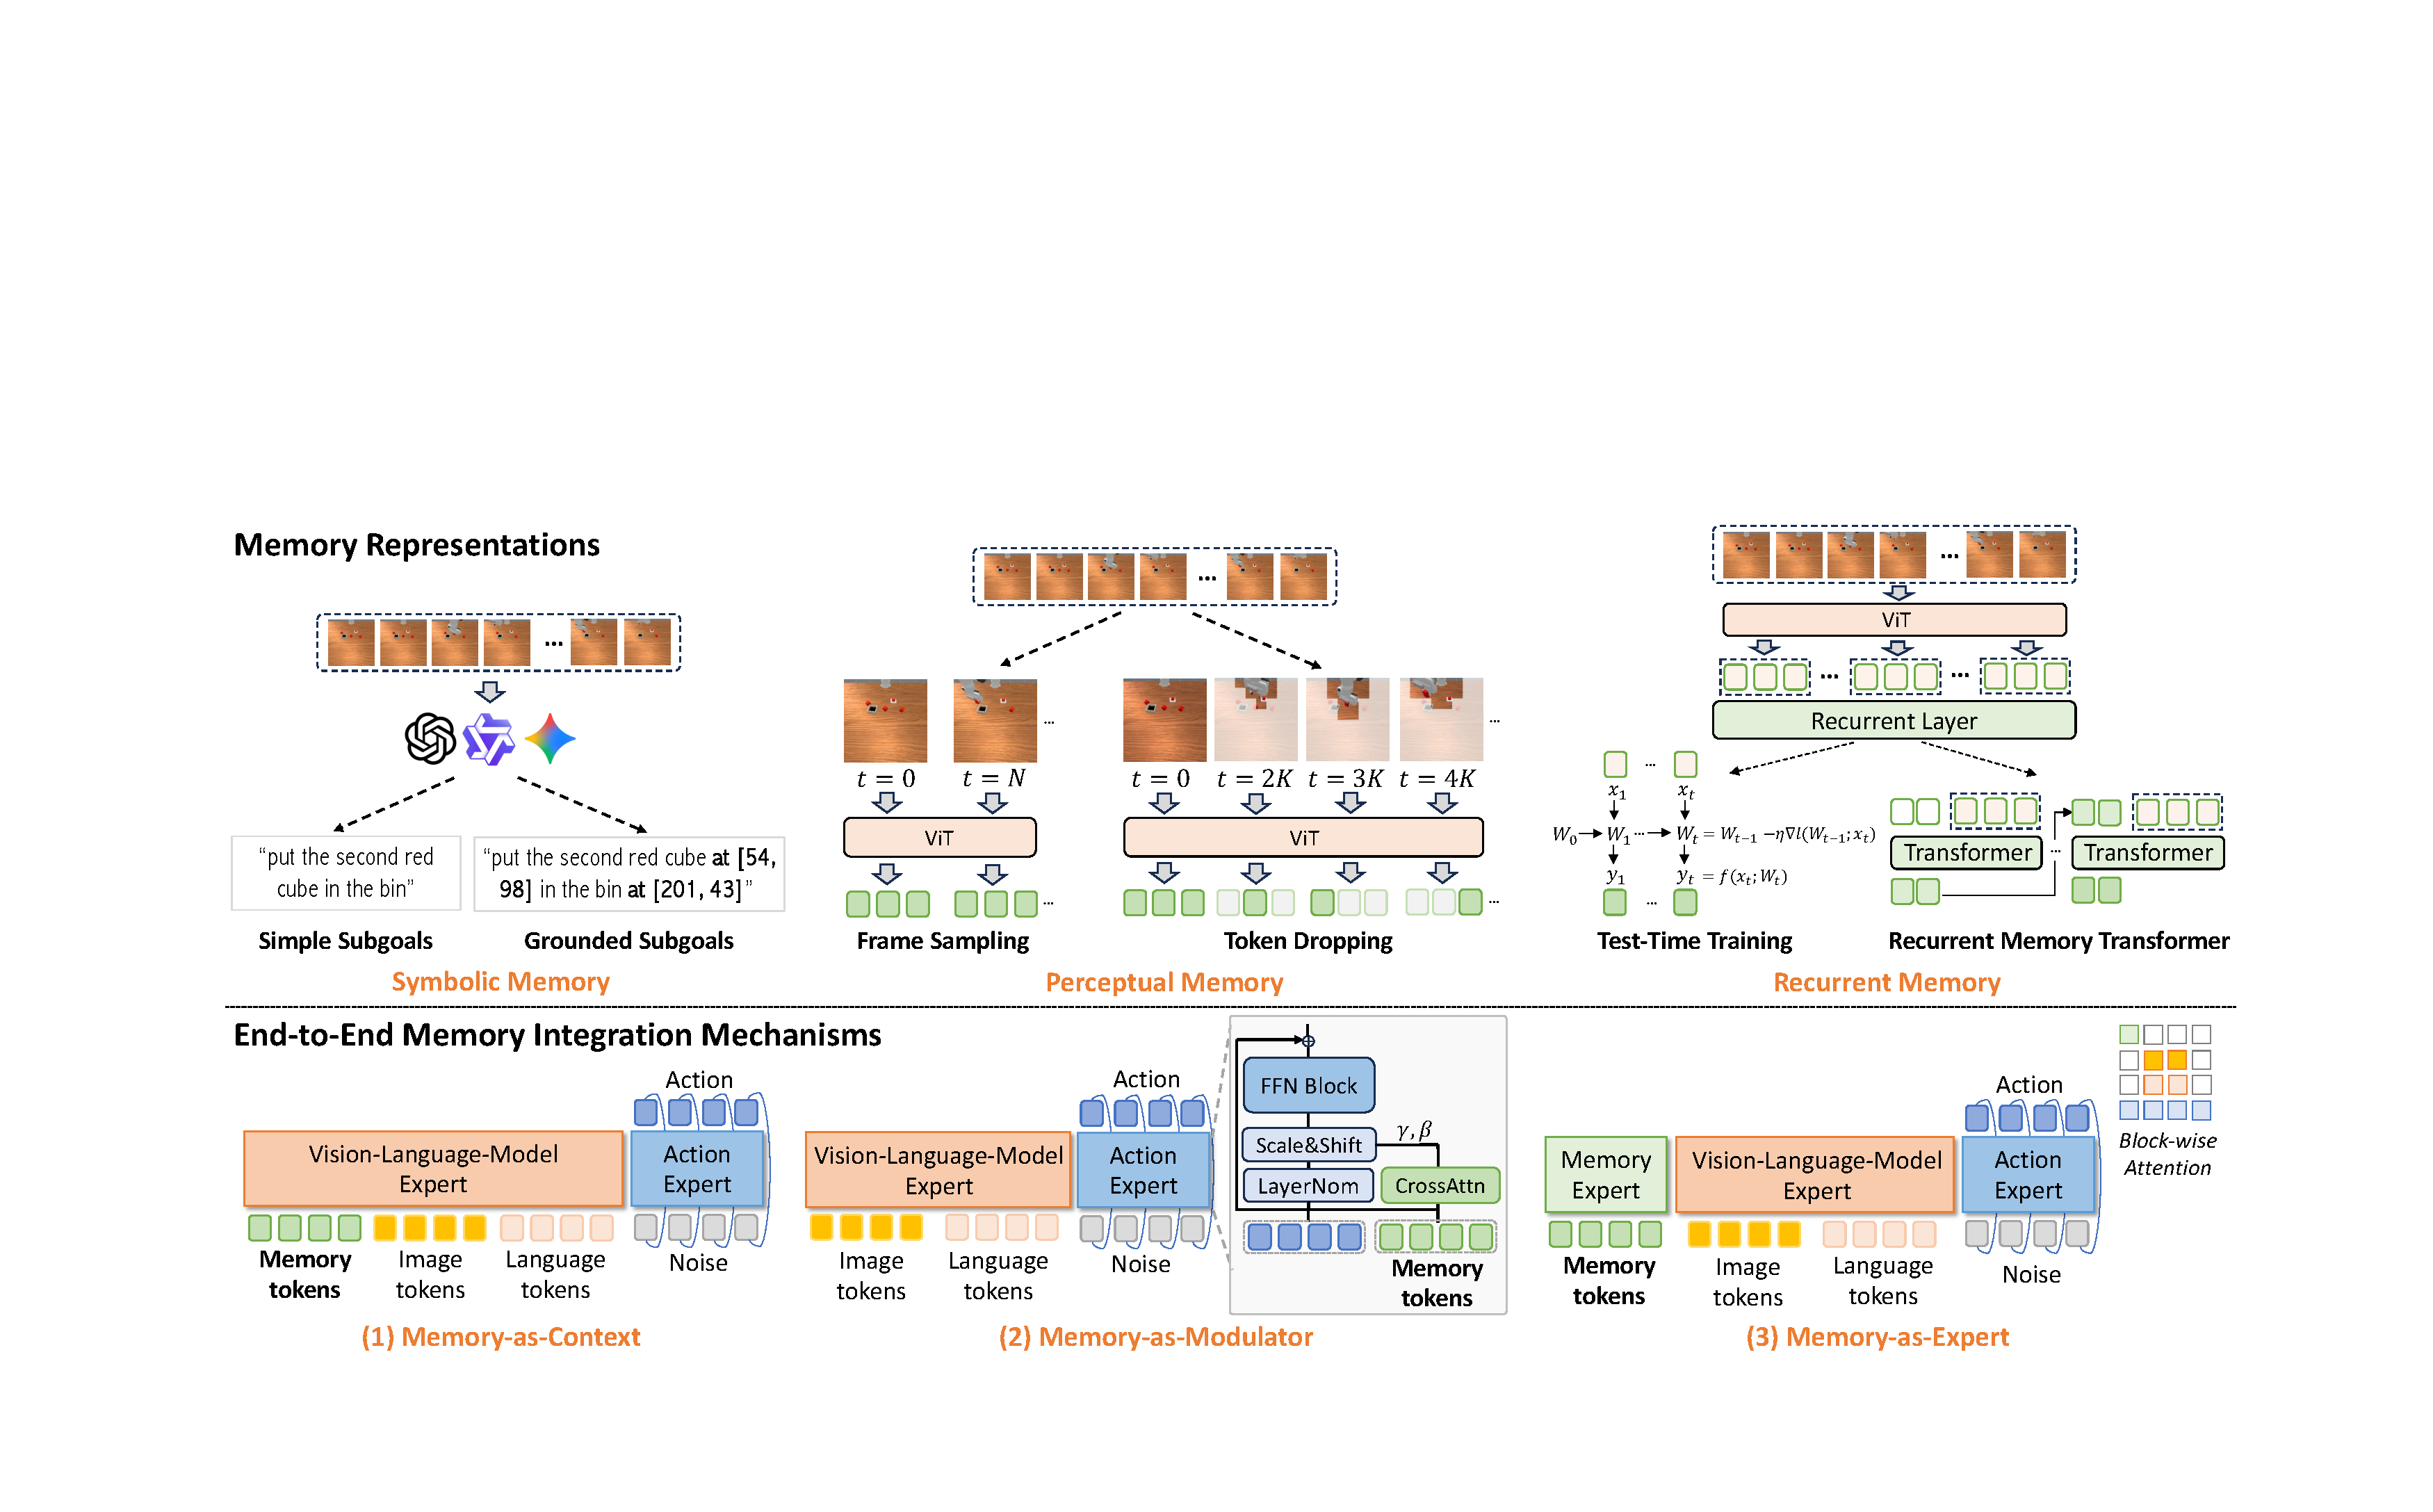
\includegraphics[width=\linewidth]{images/model_design.pdf}
    \caption{\textbf{Framework of \modelname\xspace Suite.} 
    The top part illustrates three memory representations, each with two instantiations: (1) \textit{Symbolic Memory} summarizes past interactions as high-level abstractions via language-based subgoals, optionally grounded to image pixels; (2) \textit{Perceptual Memory} encodes history as raw visual tokens,  using either token dropping to remove redundancy or uniform frame sampling to preserve essential context; (3) \textit{Recurrent Memory} compresses history into fixed-size latent states through test-time training or recurrent memory transformers.
    The bottom part shows three integration strategies consistent with $\pi_{0.5}$:
    (1) \textit{Memory-as-Context} concatenates memory tokens with observation tokens (e.g., images, task instructions, and proprioception);
    (2) \textit{Memory-as-Modulator} applies adaptive LayerNorm to modulate the action expert, where action features cross-attend to memory tokens via multi-head attention;
    (3) \textit{Memory-as-Expert} adds a separate memory expert that interacts with other experts through block-wise causal attention.
    }
    \label{fig:memory_design}
    % \vspace{-5pt}
\end{figure*}

\subsection{Benchmark Construction}

We build on the ManiSkill simulator~\cite{mu2021maniskill} using a tabletop environment with a 7-DOF Franka Panda arm. 
Training episodes are generated by replaying predefined keyframe waypoints and are recorded as dense trajectories.


\noindent\textbf{Observations and Actions.}
At each timestep, the robot receives multi-view RGB observations from front- and wrist-mounted cameras (both $256 \times 256$), along with proprioceptive states including joint positions, end-effector (EEF) pose, and gripper state. The action space is defined in either absolute joint space or absolute EEF space: joint-space actions are 8D (7 joints + gripper), EEF-space actions are 7D (3D position, Euler orientation, and gripper).
Tasks in the \TSfour\xspace suite and those prefixed with ``Video'' use video-based observations (a sequence of historical frames with paired proprioception) at the initial step, whereas all other tasks use image-based observations (a single current frame with paired proprioception). During execution, all tasks provide image-based observations at every timestep.

\noindent\textbf{Data Curation.}
To enhance behavioral diversity, particularly failure recovery, which is important for imitation learning~\cite{dai2025racer}, we inject controlled perturbations during data generation by adding 5\% noise to keyframe waypoints and then recovering to the normal  trajectory. Tasks are further stratified into easy, medium, and hard levels based on scene clutter, horizon length, and environmental dynamics. To ensure data quality, we discard episodes in which the built-in planner fails, retaining only successful rollouts for training and environment seeds for evaluation. The final dataset spans 16 tasks with 100 episodes each, yielding 1,600 demonstrations and \trainsteps\xspace  timesteps. Individual episodes range from a few hundred to over one thousand steps, reflecting long-horizon, history-dependent behaviors.

\noindent\textbf{Benchmark Comparison.}
Table~\ref{tab:dataset_comparison} provides a detailed comparison with prior benchmarks. Most existing benchmarks \cite{han2025robocerebra, zhang2025vlabench, mees2022calvin} are designed to emphasize long-horizon planning and task complexity. While these tasks may implicitly require temporal reasoning, they do not explicitly enforce other types of memory, as decisions can typically be made from immediate observations alone. 
In contrast, \benchname\xspace introduces greater environmental complexity and video-conditioned tasks, and is the first to systematically cover four types of memory: temporal\footnote{The taxonomy in MIKASA \cite{cherepanov2025memory} defines concepts such as sequential memory and memory capacity, which can be viewed as specific instances of our broader notion of temporal memory.}, spatial, object, and procedural. This design enables a more comprehensive evaluation of memory-augmented robotic policies.